\par
Avant d’investir des millions de dollars et des centaines d’heures pour 
construire un bâtiment, les propriétaires fonciers doivent savoir si le 
plancher peut supporter le bâtiment en question. Un sous-sol mou et 
rempli d'air peut conduire à un dépôt plus fort que souhaité, ce qui 
conduit à des fissures prématurées dans tout le bâtiment.
\par
De ce fait, le plus sage est de recourir au préalable à des études de sol.   
Malgré la valeur que peut coûter de telles études, que ce soit en termes
économique et/ou temporel, les caractéristiques d’un sol restent une
information essentielle à bien des égards. De ce fait, des études sont 
réalisées lors de la construction de grandes infrastructures ou de routes. 
\par 
La zone d'étude de ce projet correspond à Haïti. 
Cette île située dans les Caraïbes a une superficie de  \SI{27750}{\kilo\metre\squared}.
\begin{figure}
    \centering
    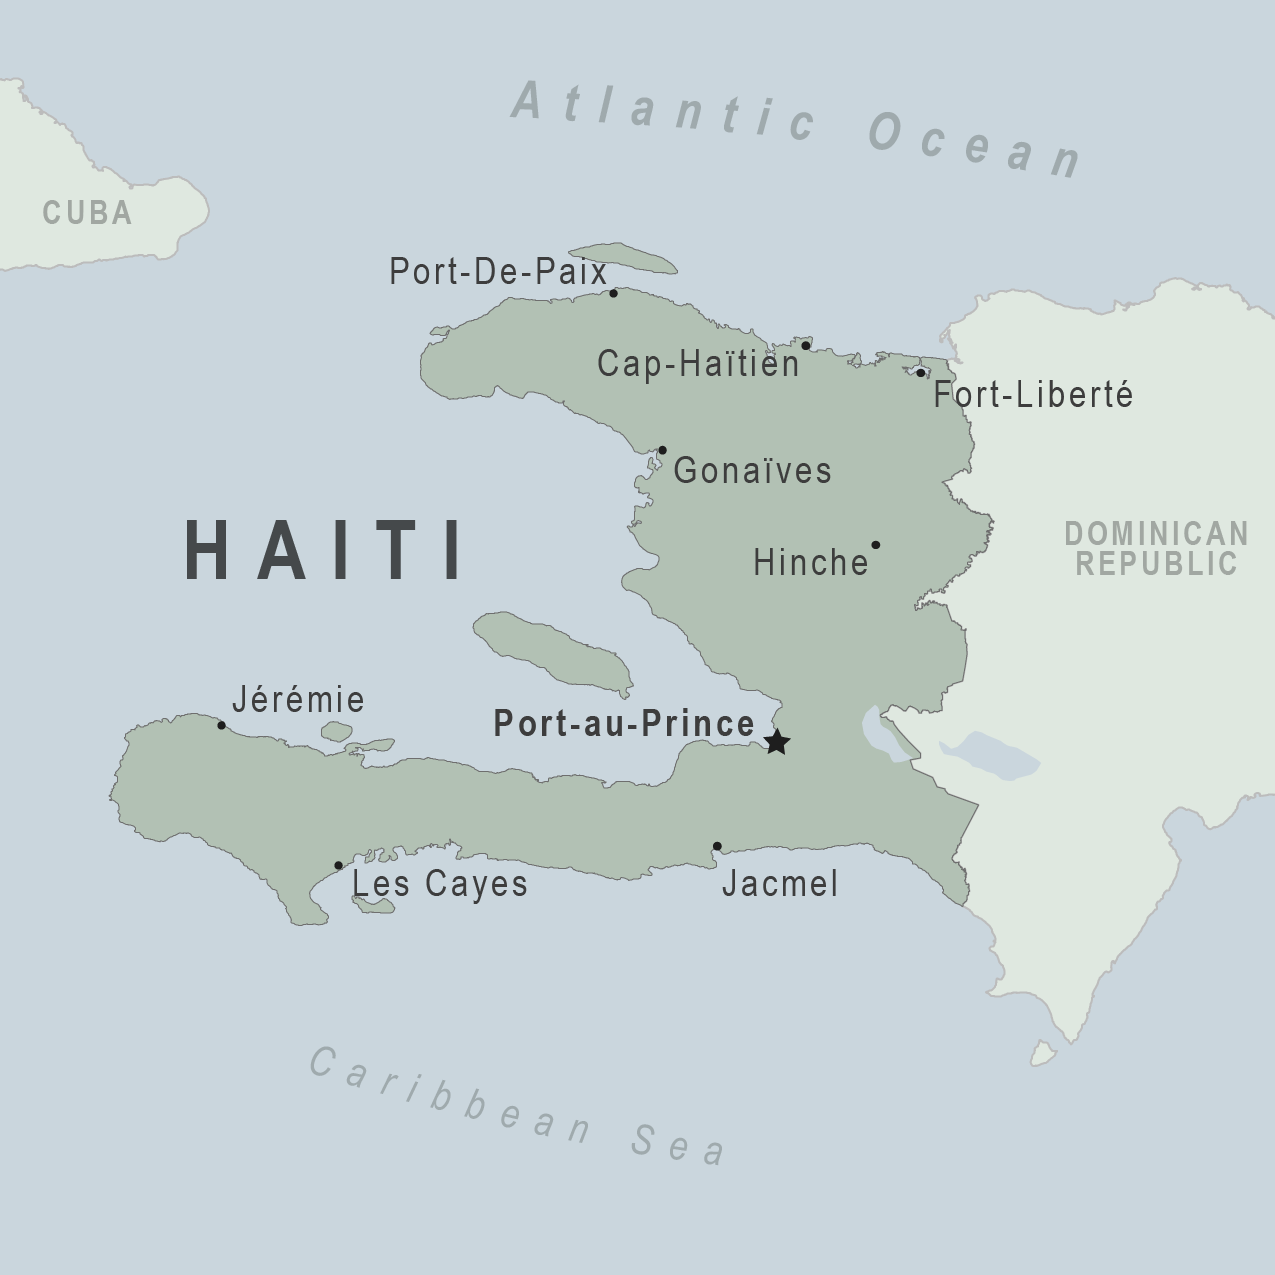
\includegraphics[width=1\textwidth]{map-haiti.png}
    \caption{Cartographie d'Haïti}
\end{figure}